We report on the application of our method for surveillance synthesis to two case studies. We have implemented the simulation in \texttt{Python}, using the \texttt{slugs} reactive synthesis tool~\cite{EhlersR16}. The experiments were performed on an Intel i5-5300U 2.30 GHz CPU with 8 GB of RAM. 

\subsection{Liveness surveillance specification + task specification}
Figure~\ref{fig:case1} shows a gridworld divided into  'rooms'. The surveillance objective requires the agent to infinitely often know precisely the location of the target (either see it, or have a belief consisting of one cell). Additionally, it has to perform the task of patrolling (visiting infinitely often) the green 'goal' cell. Formally, the specification is $\LTLglobally\LTLfinally p_1 \wedge \LTLglobally\LTLfinally \mathit{goal}$. The agent can move between $1$ and $3$ cells at a time. The sensor model used here is 'line-of-sight' with a range of 5 cells. The agent cannot see through obstacles (shown in red) and cannot see further than 5 cells. 


\begin{figure}
\subfloat[Gridworld with a user provided abstraction with 7 abstract belief states marked in black lines. \label{fig:case1}]{
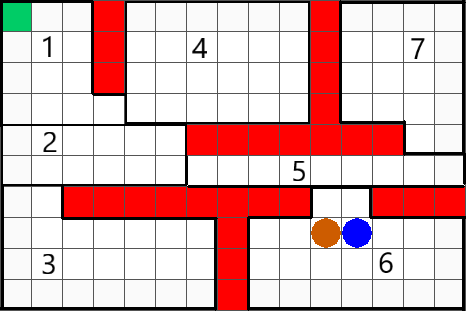
\includegraphics[scale=0.3]{figs/Liveness_part.png}
}
\hfill
\subfloat[Gridworld showing visibility of the agent. All states in black are invisible to the agent. \label{fig:case1vis}]{
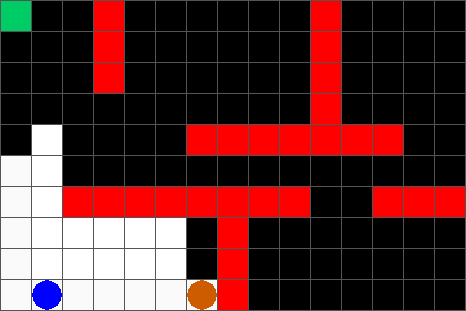
\includegraphics[scale=0.3]{figs/Liveness_t1.png}\hspace{.5cm}
}

\caption{10x15 gridworld with a surveillance liveness specification. The agent is blue, and the target to be surveilled is orange. Red states are obstacles.}
\label{fig:casestudies}

\end{figure}



Using the 7 abstract states as shown in Figure \ref{fig:case1}, the overall number of states in the two-player game is $15\times10 + 2^7 = 278$ states. In contrast, solving the full abstract game will have in the order of $2^{150}$ states, which is a state-space size that state-of-the-art synthesis tools cannot handle. 

\begin{figure}
\begin{minipage}{5.0cm}
	\centering
		\subfloat[$t_1$ \label{fig:case1t2}]{
		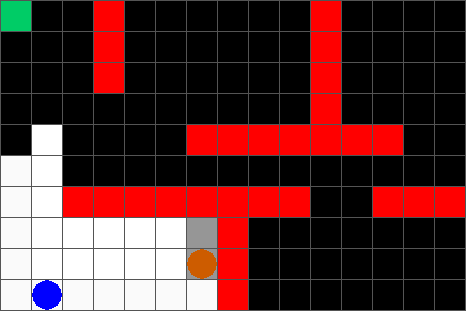
\includegraphics[scale=0.17]{figs/Liveness_t2.png}\hspace{.5cm}
	}
	\subfloat[$t_3$ \label{fig:case1t3}]{
		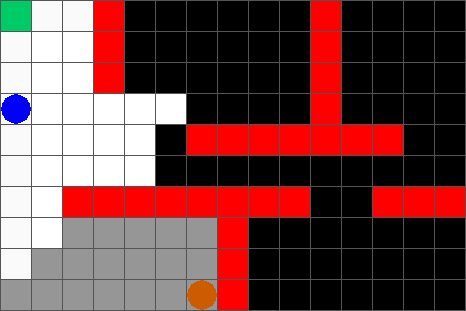
\includegraphics[scale=0.17]{figs/Liveness_t3.png}\hspace{.5cm}
	}
	\subfloat[$t_4$ \label{fig:case1t4}]{
	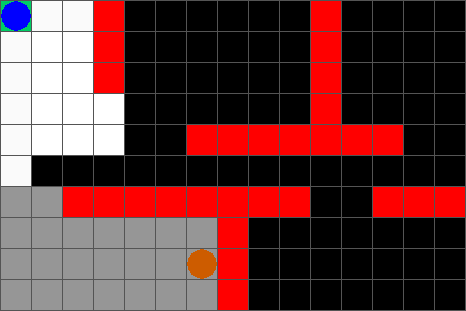
\includegraphics[scale=0.17]{figs/Liveness_t4.png}\hspace{.5cm}
}
\end{minipage}
\begin{minipage}{5.0cm}
	\centering
	\subfloat[$t_5$  \label{fig:case1t5}]{
		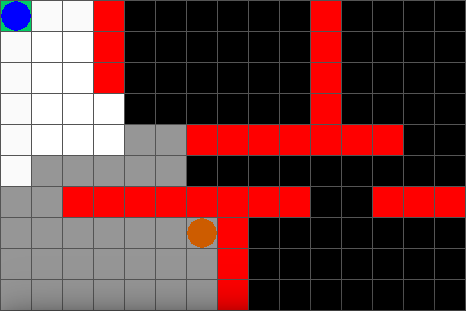
\includegraphics[scale=0.17]{figs/Liveness_t5.png}\hspace{.5cm}
	}
	\subfloat[$t_6$ \label{fig:case1t6}]{
		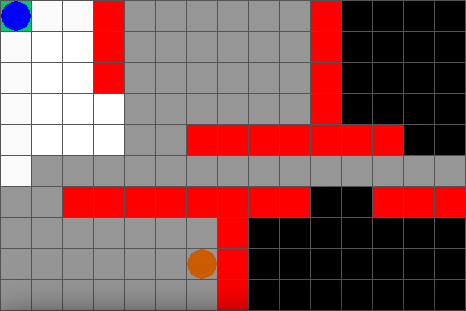
\includegraphics[scale=0.17]{figs/Liveness_t6.png}\hspace{.5cm}
	}
	\subfloat[$t_7$ \label{fig:case1t7}]{
		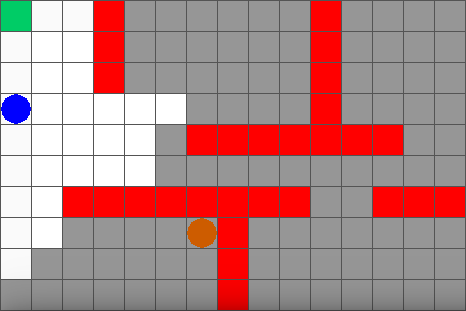
\includegraphics[scale=0.17]{figs/Liveness_t7.png}\hspace{.5cm}
	}
	
\end{minipage}

	
	\caption{Evolution of the agent's belief in target location as it moves to the goal and loses sight of the target. Grey states represents the states the agent believes the target could be in. We show the belief at different timesteps (note that $t_2$ is excluded for space concerns)
		}
	\label{fig:case1exp}
	
\end{figure}

Figure \ref{fig:case1exp} shows how when the agent cannot see the target, the belief (shown in grey) can grow quickly. This growth occurs due to the coarseness of the abstraction, which overapproximates the target's true position. In 7 timesteps, the agent believes the target can exist anywhere in the grid that is not in its vision. It has to then find the target in order to satisfy the surveillance requirement. In this example, 7 abstract states were enough to guarantee the satisfaction surveillance specification, but for comparison, we also solve the game with 12 abstract states to illustrate the change in growth in belief. Figure \ref{fig:case1fineexp} shows the belief states growing much more slowly as the abstract belief states are smaller so it more closely approximates the true belief.

\begin{figure}
	\begin{minipage}{5.0cm}
		\centering
		\subfloat[$t_1$ \label{fig:casefine1t2}]{
			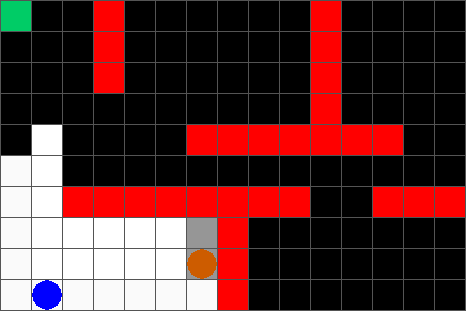
\includegraphics[scale=0.17]{figs/Liveness_t2.png}\hspace{.5cm}
		}
		\subfloat[$t_3$ \label{fig:case1finet3}]{
			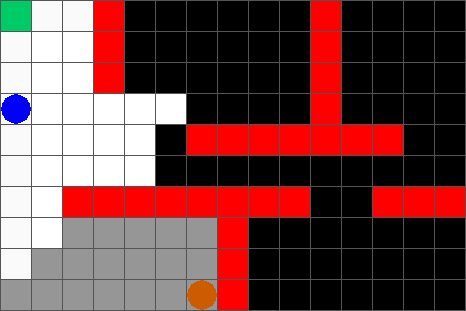
\includegraphics[scale=0.17]{figs/Liveness_t3.png}\hspace{.5cm}
		}
		\subfloat[$t_4$ \label{fig:case1finet4}]{
			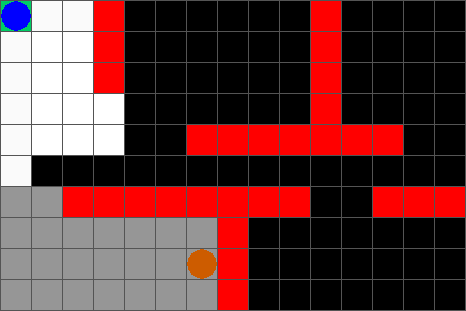
\includegraphics[scale=0.17]{figs/Liveness_t4.png}\hspace{.5cm}
		}
	\end{minipage}
	\begin{minipage}{5.0cm}
		\centering
		\subfloat[$t_5$  \label{fig:case1finet5}]{
			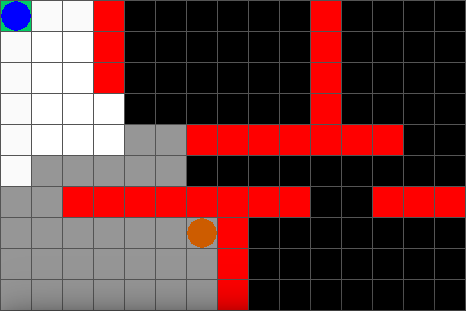
\includegraphics[scale=0.17]{figs/Liveness_t5.png}\hspace{.5cm}
		}
		\subfloat[$t_6$ \label{fig:case1finet6}]{
			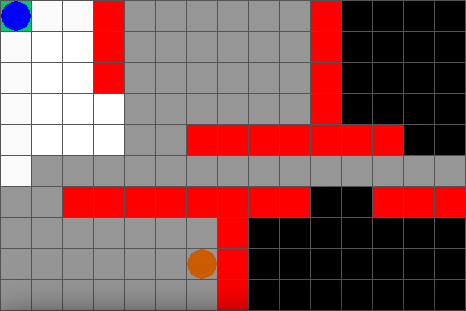
\includegraphics[scale=0.17]{figs/Liveness_t6.png}\hspace{.5cm}
		}
		\subfloat[$t_7$ \label{fig:case1finet7}]{
			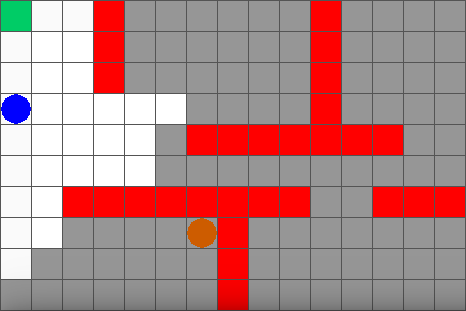
\includegraphics[scale=0.17]{figs/Liveness_t7.png}\hspace{.5cm}
		}
		
	\end{minipage}
	
	
	\caption{Evolution of the agent's belief in target location when the game is solved with 12 abstract belief states.
	}
	\label{fig:case1fineexp}
	
\end{figure}

%Starting with an abstract game with 104 states generated by a partition with four elements, our refinement algorithm terminates after 5 iterations (with total running time of 821 s). The resulting partition $\mathcal{Q} = \{Q_1,...,Q_9 \}$ has $9$ elements shown as the numbered regions in Figure~\ref{fig:case1}. Thus, the final refined abstract game has $616$ abstract states ($2^9$ abstract belief states). In contrast, the belief-set game structure would have in the order of $2^{100}$ states, which is a state-space size that state-of-the-art synthesis tools cannot handle.


%The refinement algorithm terminates after 5 iterations to produce the abstract partition  corresponding to the numbered sets in figure . There are 9 belief states which results in an additional $2^9 = 512$ states to the full observation game which is far lower than the full reduction which will be a power set of all 104 states.

The additional abstract belief states results in a much larger game as the state space grows exponentially in the number of abstract belief states. Table \ref{tab:exp1} compares the state spaces and the amount of time it takes to synthesize a controller.


\begin{table}[h!]
	\centering
	\begin{tabular}{c|c|c}
		Abstract states & Total states & Synthesis time \\ \hline \hline
		7 & 278 & 37s \\ 
		12 & 4346 & 527s \\ 
	\end{tabular}\caption{Comparison of synthesis times for the two cases} \label{tab:exp1}
\end{table}


A video simulation can be found at \url{http://goo.gl/YkFuxr}. Note the behaviour of the agent - visiting the goal and then searching for the target. This contrasts with the behaviour under safety surveillance which will we look at next.

\subsection{Safety surveillance specification + task specification}
%\begin{figure}
%\centering
%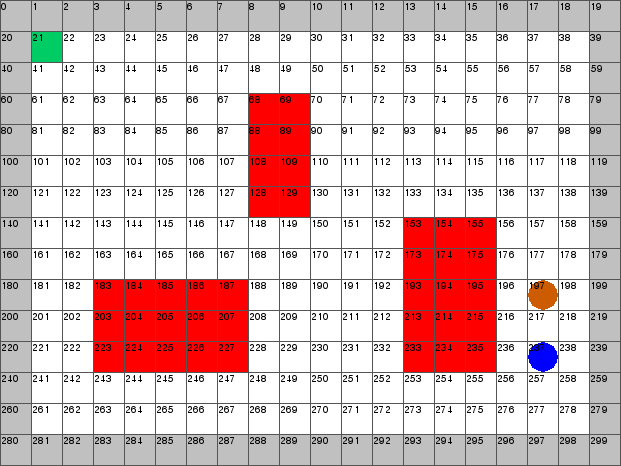
\includegraphics[scale=0.2]{case2.png}\caption{Gridworld representing an outdoor environment.}\label{fig:case2}
%\vspace{-.5cm}
%\end{figure}
Figure~\ref{fig:case2} depicts a gridworld of an 'outdoor' environment where the red blocks model buildings. 
In this setting, we enforce the safety surveillance objective $\square p_{30}$ (the belief size should never exceed 30) in addition to infinitely often reaching the green cell. The formal specification is $\LTLglobally\LTLfinally p_{30} \wedge \LTLglobally\LTLfinally \mathit{goal}$. Additionally, the target itself is trying to reach the goal cell infinitely often as well, which is known to the agent.

We used an abstraction generated by a partition of size 6, which was sufficiently precise to compute a surveillance strategy in 210 s. This demonstrates that even for larger grids, a coarse abstraction can be sufficient. Again, note that the precise belief-set game would have in the order of $2^{200}$ states.
 
We simulated the environment and the synthesized surveillance strategy for the agent in ROS. A video of the simulation can be found at \url{http://goo.gl/LyC1gQ}. Note the qualitative difference in behaviour compared to the previous example. There, in the case of liveness surveillance, the agent had more leeway to completely lose the target in order to reach its goal location, even though the requirement of reducing the size of the belief to $1$ is quite strict. Here, on the other hand, the safety surveillance objective, even with a large threshold of $30$, forces the agent to follow the target more closely, in order to prevent its belief from getting too large. The synthesis algorithm thus provides the ability to obtain qualitatively different behaviour as necessary for specific applications by combining different objectives. 

%\Suda{Not sure if we should keep this next part}
%\subsection{Discussion of behaviour}
%The difference in the behaviour in the case studies highlights the different use cases of the surveillance objectives. In more indoor settings or structured environments, a liveness surveillance objective is feasible as the agent can more easily search and find the target even if the belief grows very large. However, in outdoor environments this is harder to accomplish as the target has more room to hide. 